\subsection{Changing $\alpha_k$}

\subsubsection{Removing $\alpha_k$}\label{subsubsec:remove-alpha-k}
% Overvej om denne subsubsection er interessant nok at have med i sidste udgave af artiklen, eller om den skal i appendix.
In this experiment we changed $\alpha_k$ from $(1 / (K + 1))$ to $1$ and essentially removed the variable to see what impact it had on the results.
This method is called LightGCN-Ak1 which stands for LightGCN $\alpha_k = 1$.
This will result in the embeddings scaling more than they otherwise would have with $\alpha_k$ as normalization.
As can be seen on \autoref{fig:ndcg-yelp2020-alpha-k} and \autoref{fig:recall-yelp2020-alpha-k} changing $\alpha_k$ decreases performance of LightGCN on the yelp2020 dataset.
In the initial epochs, LightGCN-Ak1 performs better, but quickly starts to decline in performance.
On \autoref{fig:ndcg-amazon-alpha-k} and \autoref{fig:recall-amazon-alpha-k} LightGCN and LightGCN-Ak1 was run on the amazon-book dataset, but can seen that LightGCN still outperforms LightGCN-Ak1.
These results indicates that $\alpha_k$ is an important part of the layer combination for weighted summation, and we will continue our experimentation on trying to optimize $\alpha_k$
\begin{figure}
    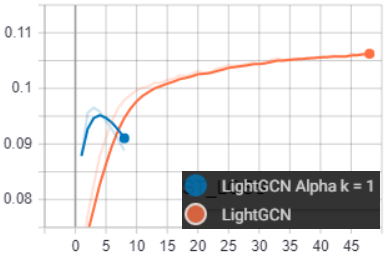
\includegraphics[width=\linewidth]{figures/alpha-k-results/yelp2020-ndcg.png}
    \caption{NDCG@50 of LightGCN and LightGCN-Ak1 on yelp2020}
    \label{fig:ndcg-yelp2020-alpha-k}
\end{figure}
\begin{figure}
    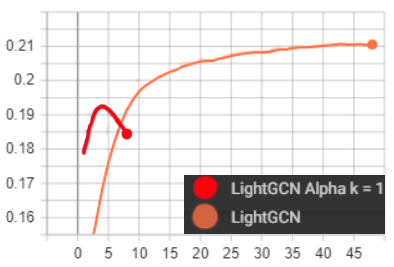
\includegraphics[width=\linewidth]{figures/alpha-k-results/yelp2020-recall.png}
    \caption{Recall@50 of LightGCN and LightGCN-Ak1 on yelp2020}
    \label{fig:recall-yelp2020-alpha-k}
\end{figure}
\begin{figure}
    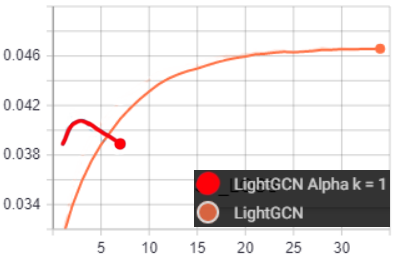
\includegraphics[width=\linewidth]{figures/alpha-k-results/amazon-ndcg.png}
    \caption{NDCG@50 of LightGCN and LightGCN-Ak1 on amazon-book}
    \label{fig:ndcg-amazon-alpha-k}
\end{figure}
\begin{figure}
    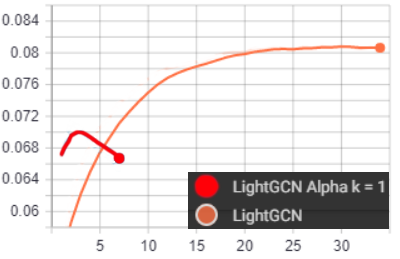
\includegraphics[width=\linewidth]{figures/alpha-k-results/amazon-recall.png}
    \caption{Recall@50 of LightGCN and LightGCN-Ak1 on amazon-book}
    \label{fig:recall-amazon-alpha-k}
\end{figure}

\subsubsection{Utilizing only one layer}
As we showed previously that removing $\alpha_k$ is harmful for performance, we want to investigate the influence of the different layers.
In this section we experiment with removing the layer combination, and only utilizing a specific convolution layer.
$\mathbf{e}^{(0)}$, $\mathbf{e}^{(1)}$, $\mathbf{e}^{(2)}$, $\mathbf{e}^{(3)}$, $\mathbf{e}^{(4)}$ and $\mathbf{e}^{(5)}$ are used as the final embeddings in each experiment respectively.

\begin{table*}[]
    \begin{tabular}{|l|l|l|l|}
        \hline
                             & Amazon-Cell-Sport  & Yelp2020           & Amazon-Book         \\ \hline
        Weighted sum (3 con) & 0.03237            & \underline{0.1064} &                     \\ \hline
        Weighted sum (4 con) &                    &                    &                     \\ \hline
        Weighted sum (5 con) &                    &                    &                     \\ \hline
        $\mathbf{e}^{(0)}$   & 0.02169            & 0.08177            & 0.03669             \\ \hline
        $\mathbf{e}^{(1)}$   & 0.02523            & 0.1019             & \textbf{0.0458}     \\ \hline
        $\mathbf{e}^{(2)}$   & 0.03419            & \textbf{0.1086}    & \underline{0.04487} \\ \hline
        $\mathbf{e}^{(3)}$   & 0.03483            & 0.09956            & 0.0372              \\ \hline
        $\mathbf{e}^{(4)}$   & \underline{0.0366} & 0.08863            & 0.03247             \\ \hline
        $\mathbf{e}^{(5)}$   & \textbf{0.03733}   & 0.0819             & 0.02923             \\ \hline
    \end{tabular}
    \centering
    \caption{Experiment on LightGCN where different layers are used as the final embedding.}
    \label{tab:only-use-one-layer-experiment}
\end{table*}